\chapter{Step 3: Uncertainty Analysis}\label{dev-step3}

\begin{abstract}
    Step 3 of an RDM-based analysis examines the performance of the set of non-dominated policy alternatives discovered during the policy alternative determination step across a large set of potential future states of the world (SOWs). This step is common for all three methods under consideration, with the only difference being that uncertainty analysis is repeated for each reference scenario used in multi-scenario MORDM. The first element of uncertainty analysis, computational exploration, is described in \cref{step3-explore}. In addition to exploring how each policy alternative responds to a variety of potential SOWs, the uncertainty analysis phase includes calculating the robustness of each policy based on the results of that exploration, which is discussed in \cref{step3-robust}.
\end{abstract}

\medskip

\begin{figure}[h]
    \centering
    \captionsetup{justification=centering}
    
    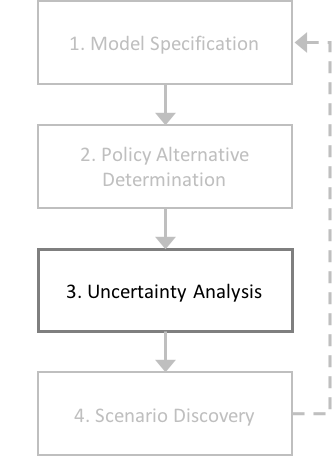
\includegraphics{structure-step3}
    \caption{RDM Structure - Step 3}
    \label{fig:structure-step3}
\end{figure}

\newpage

\section{Computational Exploration}\label{step3-explore}
The first part of uncertainty analysis, computational exploration, involves examining how each policy in the non-dominated set of alternatives behaves under an large ensemble of potential future states of the world. Remember that these alternatives were selected based on their performance in one, in the case of MORDM and multi-scenario MORDM, or only 50, in the case of MORO, scenarios. Computational experimentation, then, reveals how the identified alternatives behave given a much broader ensemble of potential future SOWs \citep{Kasprzyk2013}. 

The first part of computational exploration is to build a large ensemble of uncertainty vectors, accomplished through sampling across the uncertainty space identified in model specification. Several sampling strategies are available to build the ensemble of SOWs, including random sampling, importance sampling, and Latin Hypercube Sampling (LHS). This study makes use of LHS, as it provides an efficient way to divide the uncertainty space evenly with even a small sample size \citep{Helton2006}. The LHS technique ensures, that the entire range of each uncertainty parameter is equally represented in the sample set, which guarantees that no one uncertainty parameter is weighted more significantly in the exploration \citep{Mckay1979}. LHS is, therefore, ideal in cases involving a computationally expensive model as it can build an ensemble that describes the entire uncertainty space in with fewer scenarios than would be required with a purely random technique. 

The uncertainty space is defined in \cref{table:uncertainties}, and is sampled to build an ensemble fo 10,000 vectors of the five uncertainty parameters. Each policy from the non-dominated set of alternatives is tested against the generated ensemble of uncertainty vectors. This results in a large data set that describe how each policy behaves across the uncertainty space. That information is used in the next key part of uncertainty analysis, calculation of policy robustness. 

As a note, the individual sets of non-dominated policy alternatives generated in the second step of multi-scenario MORDM are evaluated separately for computational exploration, and result in separate results. 

\section{Robustness Calculation}\label{step3-robust}
Now that there is a large data set that describes each policy's performance across a broad set of potential future SOWs, robustness of each policy can be calculated. At this stage, the policy analyst selects their desired robust metric, or can select more than one metric, which may reveal different features of a policy's robustness. That decision, along with the exact configuration of the selected robust metric(s), should be made in conversation with decision makers, to ensure that their preferences and goals are accounted for \citep{Kasprzyk2013}. 

In this study, one robust metric is used: domain criterion satisficing. The exact implementation and configuration of this metric is specified in \cref{step0-robust}. Fundamentally, though, domain criterion satisficing involves determining the fraction of total scenarios for which a policy achieves the specific threshold for each outcome of interest. Each outcome of interest will have a separate robustness value, making it easier to communicate conflicts and trade-offs among the outcomes.
